% Graphic for TeX using PGF
% Title: E:\git\libea\tex\img\overview.dia
% Creator: Dia v0.97.2
% CreationDate: Fri Nov 14 13:46:43 2014
% For: fedra001
% \usepackage{tikz}
% The following commands are not supported in PSTricks at present
% We define them conditionally, so when they are implemented,
% this pgf file will use them.
\ifx\du\undefined
  \newlength{\du}
\fi
\setlength{\du}{15\unitlength}
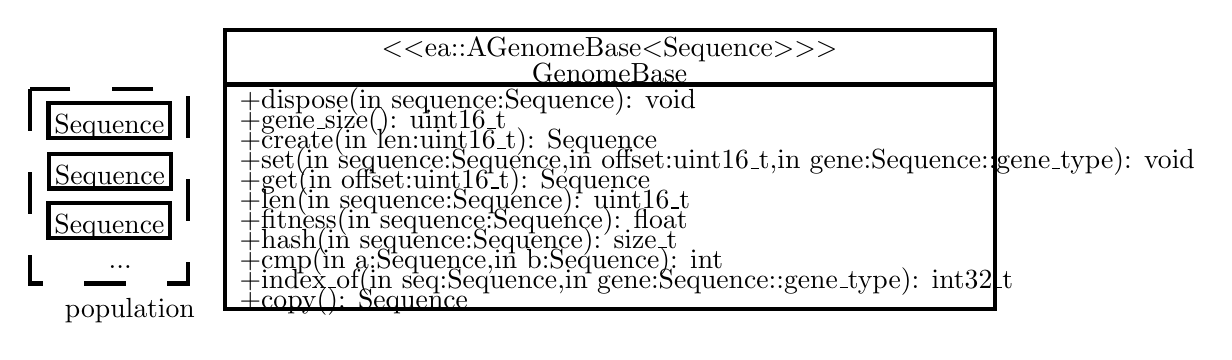
\begin{tikzpicture}[scale=0.6]
\pgftransformxscale{1.000000}
\pgftransformyscale{-1.000000}
\definecolor{dialinecolor}{rgb}{0.000000, 0.000000, 0.000000}
\pgfsetstrokecolor{dialinecolor}
\definecolor{dialinecolor}{rgb}{1.000000, 1.000000, 1.000000}
\pgfsetfillcolor{dialinecolor}
\pgfsetlinewidth{0.100000\du}
\pgfsetdash{{1.000000\du}{1.000000\du}}{0\du}
\pgfsetdash{{1.000000\du}{1.000000\du}}{0\du}
\pgfsetmiterjoin
\definecolor{dialinecolor}{rgb}{0.000000, 0.000000, 0.000000}
\pgfsetstrokecolor{dialinecolor}
\draw (18.942700\du,3.416490\du)--(18.942700\du,11.223911\du)--(25.285025\du,11.223911\du)--(25.285025\du,3.416490\du)--cycle;
\pgfsetlinewidth{0.100000\du}
\pgfsetdash{}{0pt}
\definecolor{dialinecolor}{rgb}{1.000000, 1.000000, 1.000000}
\pgfsetfillcolor{dialinecolor}
\fill (19.694000\du,3.977370\du)--(19.694000\du,5.377370\du)--(24.584000\du,5.377370\du)--(24.584000\du,3.977370\du)--cycle;
\definecolor{dialinecolor}{rgb}{0.000000, 0.000000, 0.000000}
\pgfsetstrokecolor{dialinecolor}
\draw (19.694000\du,3.977370\du)--(19.694000\du,5.377370\du)--(24.584000\du,5.377370\du)--(24.584000\du,3.977370\du)--cycle;
% setfont left to latex
\definecolor{dialinecolor}{rgb}{0.000000, 0.000000, 0.000000}
\pgfsetstrokecolor{dialinecolor}
\node at (22.139000\du,4.927370\du){Sequence};
\pgfsetlinewidth{0.100000\du}
\pgfsetdash{}{0pt}
\definecolor{dialinecolor}{rgb}{1.000000, 1.000000, 1.000000}
\pgfsetfillcolor{dialinecolor}
\fill (19.715600\du,6.007280\du)--(19.715600\du,7.407280\du)--(24.605600\du,7.407280\du)--(24.605600\du,6.007280\du)--cycle;
\definecolor{dialinecolor}{rgb}{0.000000, 0.000000, 0.000000}
\pgfsetstrokecolor{dialinecolor}
\draw (19.715600\du,6.007280\du)--(19.715600\du,7.407280\du)--(24.605600\du,7.407280\du)--(24.605600\du,6.007280\du)--cycle;
% setfont left to latex
\definecolor{dialinecolor}{rgb}{0.000000, 0.000000, 0.000000}
\pgfsetstrokecolor{dialinecolor}
\node at (22.160600\du,6.957280\du){Sequence};
\pgfsetlinewidth{0.100000\du}
\pgfsetdash{}{0pt}
\definecolor{dialinecolor}{rgb}{1.000000, 1.000000, 1.000000}
\pgfsetfillcolor{dialinecolor}
\fill (19.696300\du,7.992870\du)--(19.696300\du,9.392870\du)--(24.586300\du,9.392870\du)--(24.586300\du,7.992870\du)--cycle;
\definecolor{dialinecolor}{rgb}{0.000000, 0.000000, 0.000000}
\pgfsetstrokecolor{dialinecolor}
\draw (19.696300\du,7.992870\du)--(19.696300\du,9.392870\du)--(24.586300\du,9.392870\du)--(24.586300\du,7.992870\du)--cycle;
% setfont left to latex
\definecolor{dialinecolor}{rgb}{0.000000, 0.000000, 0.000000}
\pgfsetstrokecolor{dialinecolor}
\node at (22.141300\du,8.942870\du){Sequence};
% setfont left to latex
\definecolor{dialinecolor}{rgb}{0.000000, 0.000000, 0.000000}
\pgfsetstrokecolor{dialinecolor}
\node[anchor=west] at (21.660800\du,10.549200\du){...};
% setfont left to latex
\definecolor{dialinecolor}{rgb}{0.000000, 0.000000, 0.000000}
\pgfsetstrokecolor{dialinecolor}
\node[anchor=west] at (19.900600\du,12.303500\du){population};
\pgfsetlinewidth{0.100000\du}
\pgfsetdash{}{0pt}
\definecolor{dialinecolor}{rgb}{1.000000, 1.000000, 1.000000}
\pgfsetfillcolor{dialinecolor}
\fill (26.766600\du,1.034775\du)--(26.766600\du,3.234775\du)--(57.681600\du,3.234775\du)--(57.681600\du,1.034775\du)--cycle;
\definecolor{dialinecolor}{rgb}{0.000000, 0.000000, 0.000000}
\pgfsetstrokecolor{dialinecolor}
\draw (26.766600\du,1.034775\du)--(26.766600\du,3.234775\du)--(57.681600\du,3.234775\du)--(57.681600\du,1.034775\du)--cycle;
% setfont left to latex
\definecolor{dialinecolor}{rgb}{0.000000, 0.000000, 0.000000}
\pgfsetstrokecolor{dialinecolor}
\node at (42.224100\du,1.834775\du){\textless\textless ea::AGenomeBase\textless Sequence\textgreater\textgreater\textgreater};
% setfont left to latex
\definecolor{dialinecolor}{rgb}{0.000000, 0.000000, 0.000000}
\pgfsetstrokecolor{dialinecolor}
\node at (42.224100\du,2.784775\du){GenomeBase};
\definecolor{dialinecolor}{rgb}{1.000000, 1.000000, 1.000000}
\pgfsetfillcolor{dialinecolor}
\fill (26.766600\du,3.234775\du)--(26.766600\du,12.234775\du)--(57.681600\du,12.234775\du)--(57.681600\du,3.234775\du)--cycle;
\definecolor{dialinecolor}{rgb}{0.000000, 0.000000, 0.000000}
\pgfsetstrokecolor{dialinecolor}
\draw (26.766600\du,3.234775\du)--(26.766600\du,12.234775\du)--(57.681600\du,12.234775\du)--(57.681600\du,3.234775\du)--cycle;
% setfont left to latex
\definecolor{dialinecolor}{rgb}{0.000000, 0.000000, 0.000000}
\pgfsetstrokecolor{dialinecolor}
\node[anchor=west] at (26.916600\du,3.934775\du){+dispose(in sequence:Sequence): void};
% setfont left to latex
\definecolor{dialinecolor}{rgb}{0.000000, 0.000000, 0.000000}
\pgfsetstrokecolor{dialinecolor}
\node[anchor=west] at (26.916600\du,4.734775\du){+gene\_size(): uint16\_t};
% setfont left to latex
\definecolor{dialinecolor}{rgb}{0.000000, 0.000000, 0.000000}
\pgfsetstrokecolor{dialinecolor}
\node[anchor=west] at (26.916600\du,5.534775\du){+create(in len:uint16\_t): Sequence};
% setfont left to latex
\definecolor{dialinecolor}{rgb}{0.000000, 0.000000, 0.000000}
\pgfsetstrokecolor{dialinecolor}
\node[anchor=west] at (26.916600\du,6.334775\du){+set(in sequence:Sequence,in offset:uint16\_t,in gene:Sequence::gene\_type): void};
% setfont left to latex
\definecolor{dialinecolor}{rgb}{0.000000, 0.000000, 0.000000}
\pgfsetstrokecolor{dialinecolor}
\node[anchor=west] at (26.916600\du,7.134775\du){+get(in offset:uint16\_t): Sequence};
% setfont left to latex
\definecolor{dialinecolor}{rgb}{0.000000, 0.000000, 0.000000}
\pgfsetstrokecolor{dialinecolor}
\node[anchor=west] at (26.916600\du,7.934775\du){+len(in sequence:Sequence): uint16\_t};
% setfont left to latex
\definecolor{dialinecolor}{rgb}{0.000000, 0.000000, 0.000000}
\pgfsetstrokecolor{dialinecolor}
\node[anchor=west] at (26.916600\du,8.734775\du){+fitness(in sequence:Sequence): float};
% setfont left to latex
\definecolor{dialinecolor}{rgb}{0.000000, 0.000000, 0.000000}
\pgfsetstrokecolor{dialinecolor}
\node[anchor=west] at (26.916600\du,9.534775\du){+hash(in sequence:Sequence): size\_t};
% setfont left to latex
\definecolor{dialinecolor}{rgb}{0.000000, 0.000000, 0.000000}
\pgfsetstrokecolor{dialinecolor}
\node[anchor=west] at (26.916600\du,10.334775\du){+cmp(in a:Sequence,in b:Sequence): int};
% setfont left to latex
\definecolor{dialinecolor}{rgb}{0.000000, 0.000000, 0.000000}
\pgfsetstrokecolor{dialinecolor}
\node[anchor=west] at (26.916600\du,11.134775\du){+index\_of(in seq:Sequence,in gene:Sequence::gene\_type): int32\_t};
% setfont left to latex
\definecolor{dialinecolor}{rgb}{0.000000, 0.000000, 0.000000}
\pgfsetstrokecolor{dialinecolor}
\node[anchor=west] at (26.916600\du,11.934775\du){+copy(): Sequence};
\end{tikzpicture}
